\documentclass[kulak]{kulakarticle} % options: kulak (default) or kul

\usepackage[dutch]{babel}
\usepackage{amsmath}
\usepackage{amssymb}
\usepackage{latexsym}

\title{Project: Bipartitie Drawing Problem}
\author{Flor De Meulemeester}
\date{Academiejaar 2024 - 2025}
\address{
    \textbf{Groep Wetenschap \& Technologie Kulak} \\
    Informatica \\
    Gegevensstructuren \& Algoritmen
}

\begin{document}

\maketitle

\tableofcontents

\section*{Inleiding}

In dit verslag zullen we het \textit{Bipartite Drawing Problem} (BDP) implementeren en oplossen met enkele (meta)heuristieken. We behandelen de volgende heuristieken: 
\begin{itemize}
    \item Barycenter (BS)
    \item Splitting (SP)
    \item Tabu Search (TS) (een meta heuristiek)
\end{itemize}
Eerst bespreken we het ontwerp van deze heuristieken, vervolgens bespreken we de implementatie en ten slotte vergelijken we de heuristieken met elkaar.

\clearpage

\section{Probleemstelling} \label{chapter:probleemstelling}

Gegeven een bipartiete graaf $G(V,E)$ met twee disjuncte verzamelingen van knopen namelijk $A$ en $B$ zodat er enkel bogen zijn tussen knopen uit $A$ naar $B$ of omgekeerd. Iets formeler: Neem willekeurig $a \in A$ en willekeurig $b \in B$ dan zijn alle bogen van de vorm $(a,b) \in E$ en we hebben ook dat $V = A \cup B$ en $A \cap B = \emptyset$. We zetten de knopen in $A$ allemaal op één rechte en alle knopen uit $B$ op een andere evenwijdige rechte. Het doel is nu om het aantal kruisingen tussen de verschillende bogen te minimaliseren. \\

\noindent Dit probleem is NP-compleet en de optimale oplossing zoeken met een exact algoritme is niet aangewezen, vaak kunnen we dicht genoeg komen bij de optimale oplossing door middel van (meta)heuristieken. Met (meta)heuristieken zullen we telkens kleine aanpassingen maken aan de huidige oplossing om zo tot een kleiner aantal kruisingen te komen. Het idee bij de meeste (meta)heuristieken voor BDP is om telkens wat aanpassingen te doen in $A$, vervolgens wat aanpassingen in $B$ en dan opnieuw in $A$ en zo voort. \\

% afbeelding met een bipartiete graaf waarbij op x=0 alle knopen van A en op x=1 alle knopen van B

\noindent We definiëren eerst nog de hoogte van een knoop. We nemen hier aan dat knopen $a \in A$ op de asymptoot $x = 0$ liggen en dat knopen $b \in B$ op $x = 1$ liggen. We plaatsen nu één voor één de knopen op de asymptoten, van laag naar hoog en dus starten we met $y = 1$ en gaan zo hoger. De hoogte van een knoop is dan de y-coördinaat van die knoop. We zullen dit hier noteren als $h(a)$.

\section{Ontwerp}

In de ontwerpfase werd nagedacht over welke datastructuren de graaf konden voorstellen, hoe we het aantal kruisingen kunnen berekenen, en hoe onze heuristieken concreet moeten werken.

\subsection{Graaf voorstellen}

Het naïeve idee was om voor beide subsets een lijst met de indices bij te houden, deze indices zouden dan op hun beurt verwijzen naar een andere lijst met de indices van de buren. Op basis van de plaats in de array konden we dan de hoogte bepalen en de oplossing aanpassen en verbeteren. Indien we nu de hoogte zouden willen kijken van een knoop zouden we moeten zoeken naar de positie in de lijst. In het slechtste geval moeten we dan de volledige lijst doorzoeken. Deze operatie hebben we veel nodig en dus moest dit efficiënter. We kunnen deze lijsten vast bijhouden en zo in constante tijd de buren opvragen en dan apart een \textit{mapping} bijhouden van indices op de hoogte. Zo kunnen de operaties \textit{buren van een knoop} en \textit{hoogte van een knoop} beide in constante tijd.  

\subsection{Barycenter}

Het idee van de barycenter heuristiek is om zoveel horizontale bogen te krijgen (indien de knopen op verticale rechten staan zoals besproken in \ref{chapter:probleemstelling}) omdat deze horizontale lijnen een minimale afstand afleggen en dus minder andere bogen zullen kruisen. Dit gebeurt door de \textit{BS value} te berekenen voor elke knoop in de groep. Deze waarde wordt berekent als het gemiddelde van de hoogtes van de buren. Vervolgens zullen we de groep herordenen op basis van deze waarden. \\

\noindent Indien we de \textit{BS value} van een knoop $a \in A$, met $k$ buren $b_1, b_2, ..., b_k \in B$ (en $k \in \mathbb{N}$), willen berekenen dan ziet dit er zo uit:

\begin{align*}
    \textit{BS}(a) = \frac{1}{k} \sum_{i=1}^{k} h(b_i) 
\end{align*}

\noindent Vervolgens sorteren we de lijst met knopen uit $A$ op basis van de verkregen waardes. De knoop uit $A$ met de kleinste waarde komt vooraan, degene met de tweede kleinste waarde als tweede, en zo voort. \\

\noindent We doen dit ook voor de knopen in $B$, die hebben natuurlijk buren in $A$. Zo kunnen we om de beurt de knopen in $A$ en in $B$ permuteren tot we uiteindelijk een minimaal (niet per se optimaal) aantal kruisingen vinden. 

\subsection{Splitting}

Het idee van de splitting heuristiek is om het midden te nemen en dan voor alle andere knopen te kijken of zo beter boven of onder het midden passen. Vervolgens de beste keuze behouden per knoop en dan recursief verder gaan op de 2 groepen die overblijven, eentje boven het midden en eentje onder het midden. \\

\noindent Wanneer we met splitting de knopen in $A$ willen herordenen zullen we de knoop die in het midden ligt nemen en we noemen die $a_m$. Op deze manieren kunnen we $A$ onder verdelen in twee groepen. Knopen $a$ waarvoor $h(a) < h(a_m)$ en knopen waarvoor $h(a) > h(a_m)$. Deze groepen kunnen nu nog wijzigen want voor elke knoop $a$ zullen we kijken wat er gebeurt als we wisselen met een knoop in de andere groep. Indien dit de kruisingen verbetert dan behouden we de verandering. Voor de simpliciteit zullen we dus \textit{swaps} uitvoeren, hierdoor verandert de grootte van 2 subgroepen niet. Nadat we dit gedaan hebben voor elke knoop, herhalen we het proces op de 2 groepen die we hebben gecreëerd. Tot we maar een groep hebben van één knoop, dan zal de recursie eindigen. 

% visuele weergave van splitting

\subsection{Tabu Search}

Tabu Search is gebaseerd op Local Search, hierbij zullen we een bepaalde \textit{neighbourhood move} definiëren die een bepaalde subset aanpast. In elke iteratie zullen we alle mogelijke \textit{neighbourhood moves} genereren en kijken welke move de meeste verbetering maakt aan het aantal kruisingen. We doen dit tot dat we niet meer verbeteren en zo bereiken we een lokaal minimum. \\

\noindent Het verschil met Local Search is dat we bij TS een \textit{tabulist} bijhouden, deze bevat \textit{neighbourhood moves}. Zoals de naam al zegt zullen deze moves taboe zijn. Zolang een move in de \textit{tabulist} zit kunnen we deze move niet toepassen. Hierdoor zullen we niet altijd dezelfde moves doen en is er mogelijkheid om de minimale minima te omzeilen en eventueel een globaal minimum te vinden. Met TS kunnen we ook enkele parameters meegeven. Ten eerste, hebben we een maximaal aantal iteraties, een veilig stopcriterium zodat we zeker een eindig algoritme hebben. Ten tweede hebben we de grootte van de \textit{tabulist}. Daarnaast geven we ook een initiële oplossing mee met TS, dit kan willekeurig maar dit kan bijvoorbeeld ook door eerste een andere heuristiek te gebruiken en vervolgens die oplossing aan te bieden aan TS. Tot slot, we kunnen zelf ook kiezen wat de \textit{neighbourhood move} in houdt, in dit geval kiezen we voor het wisselen van twee knopen in dezelfde subset.

\section{Implementatie}

We analyseren nu de implementatie in Java en bespreken de concrete datastructuren en belangrijke optimalisaties.

\subsection{Kruisingen berekenen}

In Java stellen we knopen van een groep voor als HashMap van een index naar een lijst van indices uit de andere groep (\texttt{verticesA} en \texttt{verticesB}). Op deze manier kunnen we in constante tijd de buren ophalen, die we vaak zullen nodig hebben om het aantal kruisingen te berekenen. \\

\noindent Vervolgens hebben we ook een lijst voor elke groep die de huidige volgorde/oplossing van de indices weergeeft (\texttt{sequenceA} en \texttt{sequenceB}). Hieruit construeren we de oplossing en kunnen we voor een index kijken welke hoogte die heeft maar dit gaat niet in constante te tijd om te zoeken waar een getal staat in de lijst. \\

\noindent Ten slotte houden we nog een HashMap bij van de indices naar de hoogte (\texttt{heightA} en \texttt{heightB}). Nu kunnen we wel de hoogte achterhalen in constante tijd wat belangrijk is want dit wordt eigenlijk altijd gebruikt voor het berekenen van de kruisingen. Met deze structuur en de methode uit \cite{martí2003heuristics} kunnen we efficiënt het aantal kruisingen berekenen.

\subsection{Barycenter}

Voor de Barycenter methode zullen we gebruik maken van beide \texttt{sequence} en \texttt{height}. Elke iteratie berekenen voor elke knoop de \textit{BS value}, waarbij we dus vaak de hoogte nodig hebben en dus \texttt{height} gebruiken. Vervolgens permuteren we de \texttt{sequence} van deze groep gebasseerd op de waarden. Achteraf passen we de hoogtes in \texttt{height} aan zodat we verder kunnen rekenen in de volgende iteratie. We houden dan een kopie bij van de \texttt{sequence} die op dat moment het beste resultaat heeft.

\subsection{Splitting}

Voor de implementatie van splitting maken we ook gebruik van \texttt{sequence} en \texttt{height}. We gebruiken twee pointers om bij te houden waar we zitten in de \texttt{sequence}. We berekenen kruisingen en voeren swaps uit met \texttt{height}. We vergelijken elke knoop met die in het midden. Indien de knoop in de boven helft zit swappen we deze met de knoop net onder het midden. Indien de knoop in de onder helft zit swappen we deze met de knoop net boven het midden. Indien de swap geen verbetering levert doen we deze nog eens, zodat die ongedaan wordt. Nadat we alle knopen overlopen hebben updaten we \texttt{sequence} en doen we recursie op de knopen hoger dan het midden en de knopen lager dan het midden. 

\subsection{Tabu Search}

Net als bij SP definiëren we een move als het wisselen van twee knopen in dezelfde subset, deze kunnen random zijn maar we kunnen dit ook inperken door bijvoorbeeld een willekeurige knoop $a$ enkel te wisselen met knopen die maar op een bepaalde afstand van $a$ liggen. Indien we alle mogelijke moves van een subset $A$ met grootte $n$ willen genereren dan bekomen we $n^2$ mogelijke combinaties, voor grote grafen zullen best de \textit{neighbourhood} inperken dus enkel kijken naar knopen die in de buurt liggen van andere en zo aanpassingen maken. \\

\noindent Concreet is een move dus een paar van twee getallen en de \textit{tabulist} zal een ArrayList zijn van deze paren. De lengte van die lijst (\textit{tabusize}) is gelijk aan de meegegeven parameter, deze parameter kunnen we eventueel schalen aan de grootte van de graaf.

\section{Experimenten} 

\subsection{GraphBase experimenten}

We testen de geïmplementeerde heuristieken op de 3 groepen van grafen die ook gebruikt werden in de oorspronkelijke paper. \cite{martí2003heuristics} Voor TS zullen we de experimenten enkele keren uitvoeren, we variëren in het aantal iteraties $i$ en we bekijken twee types \textit{neighbourhood moves} en noteren als volgt: TS\texttt{all} waarbij we alle mogelijke swaps bekijken en TS\texttt{next} waarbij alle mogelijke swaps bekijken maar enkel tussen knopen die naast elkaar liggen, dit zijn er aanzienlijk minder en dus kunnen we dan het aantal iteraties opvoeren.

\subsubsection{Eerste experiment: Grafen met 20 knopen} \label{chapter:eerste_experiment}

Dit is een specifieke groep grafen die elk 10 knopen in $A$ en 10 in $B$ hebben. De eerste 100 grafen hebben 10 bogen, de opeenvolgende 100 grafen 20 bogen en zo voort. De resultaten van dit experiment staan in Tabel \ref{tab:experiment1}. \\

\begin{table}[h]
    \centering
    \resizebox{\textwidth}{!}{\begin{tabular}{c|ccccccccc|c|c}
    \#bogen & 10 & 20 & 30 & 40 & 50 & 60 & 70 & 80 & 90 & Gemiddelde & Tijd (s) \\
    \hline
    Barycenter & 2.75 & 23.24 & 78.66 & 178.34 & 318.99 & 514.78 & 772.35 & 1102.56 & 1532.09 & 452.37 & 0.6 \\
    Splitting & 4.39 & 31.23 & 94.09 & 195.69 & 339.42 & 534.19 & 782.84 & 1096.53 & 1482.02 & 456.04 & 2.4 \\
    TS \texttt{all} ($i=10$) & 1.45 & 21.03 & 75.49 & 172.22 & 313.83 & 501.67 & 746.52 & 1043.47 & 1435.03 & 431.07 & 3.3 \\
    TS \texttt{all} ($i=50$) & 0.63 & 14.64 & 60.62 & 149.46 & 280.0 & 464.34 & 706.9 & 1008.15 & 1415.29 & 410.00 & 13.2 \\
    TS \texttt{all} ($i=100$) & 0.5 & 13.67 & 58.15 & 147.5 & 277.64 & 461.71 & 703.65 & 1006.31 & 1413.45 & 408.25 & 25.4 \\
    TS \texttt{all} ($i=250$) & 0.4 & 12.39 & 57.38 & 146.47 & 276.73 & 460.73 & 702.63 & 1005.3 & 1411.34 & 407.34 & 64.7 \\
    TS \texttt{next} ($i=1000$) & 2.3 & 30.68 & 95.98 & 203.42 & 352.46 & 543.85 & 795.01 & 1097.43 & 1475.55 & 459.67 & 16.5\\
    TS \texttt{next} ($i=2000$) & 1.68 & 28.52 & 92.56 & 198.57 & 341.29 & 534.99 & 786.13 & 1088.34 & 1468.4 & 454.05 & 32.8 \\
    TS \texttt{next} ($i=5000$) & 1.26 & 26.32 & 87.49 & 190.58 & 332.64 & 526.19 & 773.64 & 1075.91 & 1458.25 & 447.23 & 81.1
    \end{tabular}}
    \caption{Resultaten van het eerste experiment.}
    \label{tab:experiment1}
\end{table}

\begin{figure}
    \centering
    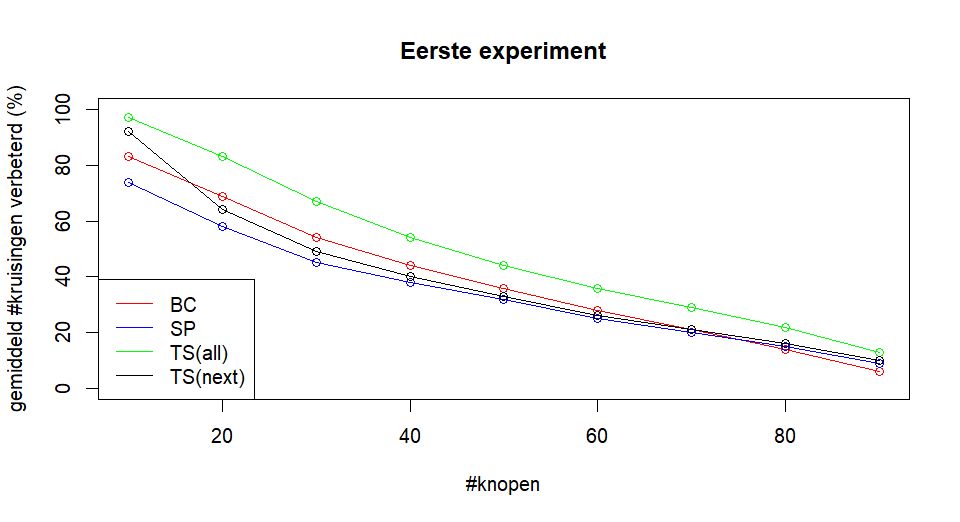
\includegraphics[width=\linewidth]{experiment1percent.png}
    \caption{De percentuele verbetering ten opzichte van het oorspronkelijk aantal kruisingen voor het eerste experiment.}
    \label{fig:exp1}
\end{figure}

\noindent De percentuele verbetering ten opzichte van het oorspronkelijk aantal kruisingen wordt weergegeven in Figuur \ref{fig:exp1}. In deze figuur staan enkel de TS\texttt{all} en TS\texttt{next} met de meeste iteraties. We zien dat onze metaheuristiek TS\texttt{all}, het altijd beter doet, zelfs met maar 10 iteraties. Dit is enigszins wel verklaarbaar want die doet ook veel meer werk en blijft doorgaan ook als we een iets slechtere oplossing tegen komen (BS zou dan stoppen). Logischer wijze doet TS nog beter als we het aantal iteraties verhogen. Indien we de \textit{neighbourhood} gaan inperken en kijken naar TS\texttt{next} en het aantal iteraties compenseren komen we niet in de buurt van TS\texttt{all}. Maar met genoeg iteraties is het toch iets beter dan BS en SP bij de grafen met meer bogen.

\subsubsection{Tweede experiment: Schaarse grafen}

De eerste 100 grafen in deze verzameling starten met 10 knopen in $A$, 10 in $B$ en met 10 knopen (dezelfde als in Figuur \ref{chapter:eerste_experiment}). De volgende 100 hebben hetzelfde aantal knopen maar nu wel 20 bogen. De 100 hierna hetzelfde aantal knopen maar nu 30 bogen en zo voort. De resultaten van dit experiment staan in Tabel\ref{tab:experiment2}. \\

\begin{table}[h]
    \centering
    \resizebox{\textwidth}{!}{\begin{tabular}{c|ccccccccc|c|c}
    \#bogen & 10 & 20 & 30 & 40 & 50 & 60 & 70 & 80 & 90 & Gemiddelde & Tijd (s) \\
    \hline
    Barycenter & 2.75 & 11.72 & 21.6 & 33.56 & 50.77 & 66.87 & 85.5 & 100.18 & 120.14 & 49.31 & 1.8 \\
    Splitting & 4.39 & 23.07 & 58.88 & 105.01 & 177.69 & 273.34 & 390.95 & 501.74 & 672.14 & 220.72 & 19.2 \\
    TS \texttt{all} ($i=10$) & 1.45 & 14.42 & 47.43 & 109.2 & 208.32 & 344.02 & 519.34 & 725.62 & 990.37 & 296.02 & 77.4 \\
    TS \texttt{all} ($i=50$) & 0.63 & 8.44 & 19.73 & 35.7 & 56.91 & 95.99 & 134.78 & 186.56 & 268.61 & 80.74 & 424.3 \\
    TS \texttt{all} ($i=100$) & 0.5 & 7.61 & 18.29 & 33.89 & 54.41 & 86.39 & 108.17 & 135.79 & 178.55 & 62.36 & 807.2 \\
    TS \texttt{all} ($i=250$) & 0.4 & 6.9 & 17.07 & 32.83 & 53.74 & 85.62 & 106.27 & 132.73 & 174.8 & 61.03 & 1792.0\\
    TS \texttt{next} ($i=1000$) & 2.3 & 54.28 & 169.95 & 323.69 & 538.05 & 801.72 & 1111.07 & 1458.86 & 1870.53 & 633.05 & 63.2 \\
    TS \texttt{next} ($i=2000$) & 1.68 & 53.8 & 169.95 & 323.69 & 538.03 & 801.6 & 1110.95 & 1458.79 & 1870.46 & 632.90 & 112.8 \\
    TS \texttt{next} ($i=5000$) & 1.26 & 53.28 & 169.86 & 323.69 & 538.01 & 801.59 & 1110.92 & 1458.76 & 1870.42 & 632.78 & 293.3 \\
    \end{tabular}}
    \caption{Resultaten van het tweede experiment.}
    \label{tab:experiment2}
\end{table}

\begin{figure}
    \centering
    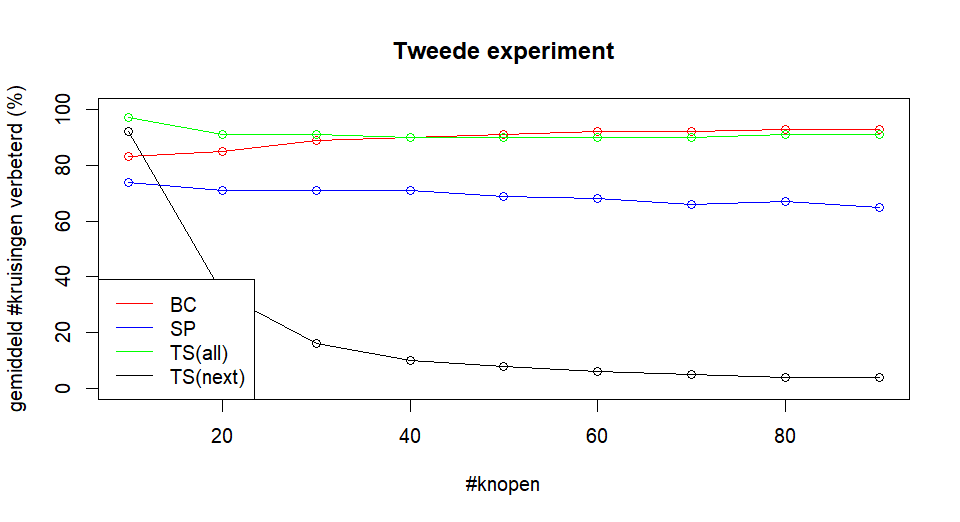
\includegraphics[width=\linewidth]{experiment2percent.png}
    \caption{De percentuele verbetering ten opzichte van het oorspronkelijk aantal kruisingen voor het tweede experiment.}
    \label{fig:exp2}
\end{figure}

\noindent De percentuele verbetering ten opzichte van het oorspronkelijk aantal kruisingen wordt weergegeven in Figuur \ref{fig:exp2}. In deze figuur staan enkel de TS\texttt{all} en TS\texttt{next} met de meeste iteraties. Bij deze spaarse grafen zien we dat BS het heel goed doet. Voor TS\texttt{all} zien we dat we met genoeg iteraties in de buurt kunnen komen van BS maar dit vergt veel meer tijd. TS\texttt{next} werkt heel slecht bij deze grafen, dit komt waarschijnlijk doordat er zo weinig knopen met elkaar verbonden zijn, de kans dat twee knopen naast elkaar beiden een graad 1 of hoger hebben redelijk klein is. Hieruit volgt dat in de meeste gevallen de swap niets zal veranderen en we een groot aantal iteraties niets doen.

\subsubsection{Derde experiment} \label{chapter:derde_experiment}

Deze grafen zijn een stuk moeilijker want ze hebben veel meer bogen ten opzichte van het aantal knopen en dat aantal knopen stijgt ook doorheen de verzameling. De eerste 100 grafen hebben 10 knopen in $A$, 10 in $B$ en 20 bogen. De opeenvolgende 100 grafen hebben 20 knopen in $A$, 20 in $B$ en 40 bogen. En zo voort. Tot 100 knopen in elke groep en 200 bogen. De resultaten van dit experiment staan in Tabel \ref{tab:experiment3}. \\

\begin{table}[h]
    \centering
    \resizebox{\textwidth}{!}{\begin{tabular}{c|cccccccccc|c|c}
    \#bogen & 20 & 40 & 60 & 80 & 100 & 120 & 140 & 160 & 180 & 200 & Gemiddelde & Tijd (s) \\
    \hline  
    Barycenter & 23.24 & 91.34 & 185.17 & 312.31 & 469.64 & 664.05 & 879.95 & 1107.53 & 1372.21 & 1707.28 & 681.27 & 18.3 \\
    Splitting & 31.23 & 148.08 & 351.03 & 639.57 & 1005.49 & 1535.76 & 2097.1 & 2792.57 & 3603.44 & 4454.79 & 1665.91 & 202.0 \\
    TS \texttt{all} ($i=10$) & 21.03 & 130.3 & 362.49 & 745.75 & 1283.12 & 1992.8 & 2853.02 & 3932.01 & 5176.89 & 6586.55 & 2308.40 & 428.51 \\
    TS \texttt{all} ($i=50$) & 14.64 & 78.57 & 191.94 & 371.16 & 618.29 & 962.78 & 1406.87 & 1948.06 & 2618.59 & 3347.97 & 1155.88 & 1892.88 \\
    TS \texttt{next} ($i=1000$) & 30.68 & 253.16 & 721.34 & 1352.36 & 2223.51 & 3305.74 & 4531.98 & 5982.62 & 7615.21 & 9486.92 & 3550.35 & 200.6 \\
    TS \texttt{next} ($i=2000$) & 28.52 & 247.96 & 720.44 & 1351.81 & 2223.49 & 3305.74 & 4531.98 & 5982.48 & 7615.16 & 9486.92 & 3549.45 & 691.3 \\
    TS \texttt{next} ($i=5000$) & 26.32 & 240.64 & 718.53 & 1351.7 & 2223.49 & 3305.71 & 4531.98 & 5982.48 & 7615.10 & 9486.92 & 3548.28 & 1535.1
    \end{tabular}}
    \caption{Resultaten van het derde experiment.}
    \label{tab:experiment3}
\end{table}

\begin{figure}
    \centering
    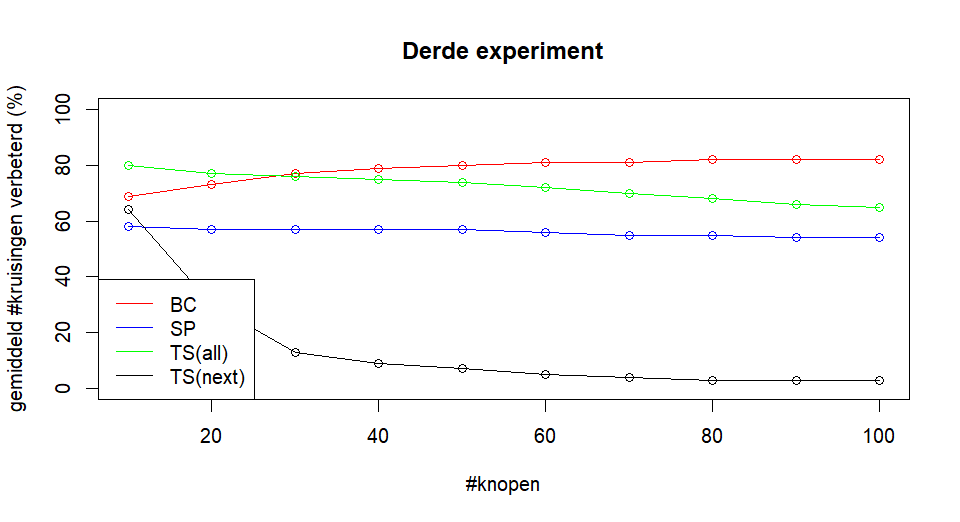
\includegraphics[width=\linewidth]{experiment3percent.png}
    \caption{De percentuele verbetering ten opzichte van het oorspronkelijk aantal kruisingen voor het derde experiment.}
    \label{fig:exp3}
\end{figure}

\noindent De percentuele verbetering ten opzichte van het oorspronkelijk aantal kruisingen wordt weergegeven in Figuur \ref{fig:exp3}. In deze figuur staan enkel de TS\texttt{all} en TS\texttt{next} met de meeste iteraties. We zien dat deze figuur heel gelijkaardig is met de vorige (Figuur \ref{fig:exp2}). We hebben hier iets minder iteraties voor TS\texttt{all} omdat het anders te lang zou duren en niet meer zo relevant zou zijn. BS is met uitsteek het best hier behalve voor de kleinere grafen. 
    
\subsection{Tabu Search}

We zagen net dat het belangrijk is om een goeie afweging te vinden tussen het aantal iteraties en de grootte van het neighbbourhood moves zodat de uitvoeringstijd niet te groot wordt en het resultaat aanvaardbaar. Nu zullen we nog de 2 andere parameters van TS onder de loep nemen.

\subsubsection{Tabusize} \label{chaper:tabusize}

We zullen de andere parameters constant houden en zullen nu de \textit{tabusize} laten variëren. Laat $n$ het aantal iteraties zijn, dan zullen we \textit{tabusize} uitdrukken als $n$ vermenigvuldigd met een $0 \leq p \leq 1$. De grootte van de \textit{tabulist} is dus $np$. Als $p=0$, dan hebben we geen \textit{tabulist} en is dit equivalent met een normale Local Search. Als $p=1$, dan doen we evenveel iteraties en zal elke move maar max 1 maal kunnen worden toegepast want ze zullen in de \textit{tabulist} blijven voor de rest van de iteratie. Voor dit experiment stellen we $n=200$ en gebruiken we dezelfde grafen als in \ref{chapter:eerste_experiment}. \\

\begin{table}[h]
    \centering
    \resizebox{\textwidth}{!}{\begin{tabular}{c|ccccccccc|c|c}
    \#bogen & 10 & 20 & 30 & 40 & 50 & 60 & 70 & 80 & 90 & Gemiddelde & Tijd (s) \\
    \hline  
    $p=0$ & 1.56 & 18.41 & 64.81 & 153.51 & 286.0 & 470.17 & 711.64 & 1010.9 & 1423.0 & 414.00 & 219.6 \\
    $p=0.01$ & 1.17 & 16.6 & 61.92 & 150.1 & 281.66 & 464.45 & 707.43 & 1009.14 & 1421.75 & 411.42 & 193.6 \\
    $p=0.1$ & 0.38 & 12.39 & 57.97 & 147.12 & 277.58 & 461.65 & 703.28 & 1005.72 & 1407.28 & 407.33 & 82.3 \\
    $p=0.25$ & 0.26 & 13.76 & 60.16 & 149.0 & 279.91 & 464.11 & 705.06 & 1008.11 & 1406.64 & 408.70 & 53.78 \\
    $p=0.5$ & 0.33 & 14.87 & 62.33 & 151.08 & 283.32 & 466.85 & 709.15 & 1010.1 & 1410.5 & 410.85 & 24.1 \\
    $p=0.75$ & 0.33 & 14.87 & 62.33 & 151.08 & 283.32 & 466.85 & 709.15 & 1010.1 & 1410.5 & 410.85 & 48.37 \\
    $p=1$ & 0.33 & 14.87 & 62.33 & 151.08 & 283.32 & 466.85 & 709.15 & 1010.1 & 1410.5 & 410.85 & 55.37
    \end{tabular}}
    \caption{Resultaten waarbij we de grootte van \textit{tabulist} laten variëren met $200p$}
    \label{tab:tabusize}
\end{table}

\noindent Voor alle experimenten hiervoor hebben we een \textit{tabusize} gelijk aan $15$ gebruikt, zodat die altijd hetzelfde was. We zien hier dat een \textit{tabusize} rond $\frac{n}{10}$ het best presteert, natuurlijk is het nog moeilijk om hier iets algemeen over te zeggen. Maar de \textit{tabusize} zal toch zeker kleiner moeten zijn dan $\frac{p}{2}$ want voor alle $p > \frac{1}{2}$ die we getest hebben lijkt TS niet veel anders te doen en niet perse beter. We zien dat $p=0.5$ wel het snelst is, dit komt waarschijnlijk omdat we dan voor een groot aantal moves niet moeten berekenen wat het verschil zal zijn in kruisingen wat nog steeds het meeste tijd neemt tijdens de uitvoering. Maar hoe komt het dan dat $p=1$ trager is, dit is waarschijnlijk omdat we ook voor elke move moeten nagaan of deze in de \textit{tabulist} zit en bij mijn implementatie gebeurt dit gewoon in een ArrayList, dus hoe groter die is, des te langer het zal duren om te checken of een move er in zit. 

\subsubsection{Start oplossing}

We voeren TS drie keer uit met dezelfde parameters maar we starten telkens met een andere initiele volgorde. De eerste keer is deze niet aangepast, de tweede keer is de startvolgorde onderworpen aan BS en de laatste keer passen we eerst SP toe op de startvolgorde. Net zoals in \ref{chaper:tabusize} gebruiken we hier 200 iteraties en we nemen de \textit{tabusize} hier op 20 (dus onze $p$ zou 0.1 zijn), dit gaf de beste oplossingen in \ref{chaper:tabusize} dus waarom niet opnieuw gebruiken. \\

\begin{table}[h]
    \centering
    \resizebox{\textwidth}{!}{\begin{tabular}{c|ccccccccc|c|c}
    \#bogen & 10 & 20 & 30 & 40 & 50 & 60 & 70 & 80 & 90 & Gemiddelde & Tijd (s) \\
    \hline  
    TS & 0.38 & 12.39 & 57.97 & 147.12 & 277.58 & 461.65 & 703.28 & 1005.72 & 1407.28 & 407.34 & 53.68 \\
    $TS_{BS}$ & 0.53 & 12.48 & 57.96 & 147.16 & 277.53 & 461.55 & 703.39 & 1005.65 & 1406.35 & 407.26 & 45.8 \\
    $TS_{SP}$ & 0.47 & 12.64 & 57.88 & 147.24 & 277.44 & 461.38 & 703.8 & 1005.46 & 1406.23 & 407.25 & 46.74
    \end{tabular}}
    \caption{We kijken naar het effect van de start oplossing voor de grafen uit \ref{chapter:eerste_experiment}.}
    \label{tab:start}
\end{table}

\noindent We zien dat de initiële oplossing niet zo'n grote invloed heeft op de waarde van onze oplossing. Maar we kunnen ook zien in Figuur \ref{tab:experiment1} dat TS toch altijd een betere oplossing bekomt dan BS en SP, indien het genoeg iteraties doet. Wat ook opvalt is dat we een snellere uitvoeringstijd hebben als we TS beginnen met een oplossing van een andere heuristiek, dit klinkt helemaal niet logisch want TS alleen doet dan toch minder werk. Een mogelijke verklaring is dat het misschien komt doordat de bottleneck nog steeds ligt bij het verschil in kruisingen berekenen tussen swaps en als we al starten met een betere oplossing dan moeten we minder kruisingen berekenen. Maar ik kan dit niet met zekerheid zeggen. \\

\noindent In het derde experiment (Figuur \ref{tab:experiment3}) kunnen we wel zien dat BS beter is. In dit geval zou het meer nut hebben om TS na BS te proberen en kijken we het nog kunnen verbeteren. Ik werd nieuwsgierig en heb dit nog even getest op de grafen uit experiment 3 (\ref{chapter:derde_experiment}). Omdat deze grafen veel moeilijker zijn, neem ik hier het aantal iteraties gelijk aan 10 en de \textit{tabusize} wordt dan 1 als we weer $p=0.1$ nemen wat goed bleek te werken uit \ref{chaper:tabusize}. Het lijkt een beetje zinloos zo'n kleine \textit{tabusize} te nemen maar hierdoor zullen we ten minste niet vast komen zitten tussen twee moves die telkens afwisselen. \\

\begin{table}[h]
    \centering
    \resizebox{\textwidth}{!}{\begin{tabular}{c|cccccccccc|c|c}
    \#bogen & 20 & 40 & 60 & 80 & 100 & 120 & 140 & 160 & 180 & 200 & Gemiddelde & Tijd (s) \\
    \hline  
    TS & 21.01 & 130.25 & 362.49 & 745.75 & 1283.12 & 1992.8 & 2853.02 & 3932.01 & 5176.89 & 6586.55 & 2308.39 & 423.1 \\
    $TS_{BS}$ & 19.21 & 83.15 & 173.75 & 298.05 & 451.11 & 640.91 & 852.46 & 1076.02 & 1336.18 & 1666.01 & 659.69 & 639.1 \\
    $TS_{SP}$ & 18.98 & 100.51 & 243.69 & 469.08 & 760.96 & 1185.05 & 1651.62 & 2247.69 & 2941.37 & 3692.12 & 1331.11 & 861.9 
    \end{tabular}}
    \caption{We kijken naar het effect van de start oplossing voor de grafen uit \ref{chapter:derde_experiment}.}
    \label{tab:start3}
\end{table}

\noindent Als we nu Tabel \ref{tab:experiment3} en Tabel \ref{tab:start3} bekijken zien we dat we onze BS oplossing van experiment 3 wel nog ietsje kunnen verbeteren als we TS er na uitvoeren. Nu is de uitvoeringstijd wel logischer, die is langer als we eerste beginnen met de oplossing van een andere heuristiek.

\section*{Besluit}

We hebben natuurlijk maar een beperkt aantal experimenten uitgevoerd en dat met een specifieke implementatie, dus de volgende uitspraken zullen misschien een beetje vertekend zijn. We zagen dat BS het altijd goed deed en heel rap, dus deze methode kunnen we beschouwen als een \textit{go-to} methode. SP deed het niet slecht maar als alternatief voor BS zouden we toch eerder moeten kijken naar TS. We zagen dat het niet vanzelfsprekend in om de goeie parameters te pakken maar als dat lukt dan is TS wel sterker mits genoeg iteraties. Voor een volgend onderzoek zouden we eventueel nog meer kunnen experimenteren met nog andere \textit{neighbourhood moves}.

\bibliographystyle{unsrt}
\bibliography{referenties.bib}
\clearpage

\end{document}
